\clearpage
\section{Manufacturing plan}
\label{appendixmanufacturing}
The table below shows the manufacturing plan. This plan was created with the help of the sandvik toolguide \cite{Sandvik}. The process step corresponds to the numbers used in Chapter \ref{manufacturing}. 
\begin{figure}[H]
\centering
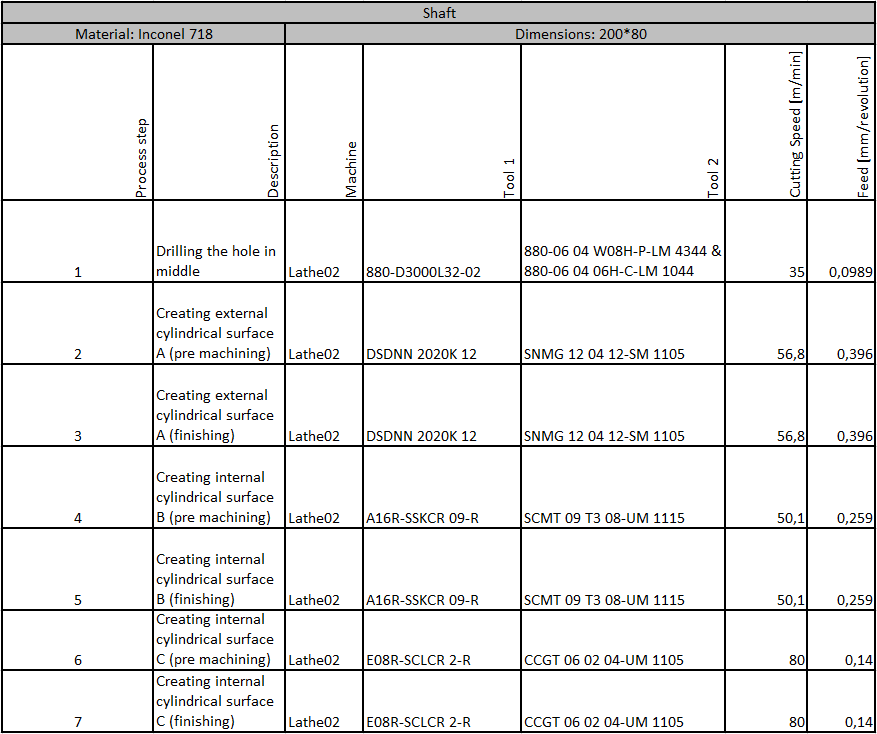
\includegraphics[width=12cm]{Figures/manufacturingtablefinal.PNG}
\caption{Manufacturing steps for the stator}
\label{manutable}
\end{figure}


\clearpage
\subsection*{Edge blends}
To create edge blend the machine has to create stair cases first and then remove those staircases in one smooth motion. This can be seen in \ref{edgeblend}. Number 1 till 4 show the staircases. For the best product these parts need to be as wide as the feed is. This prevents chip jamming. Step 5 is the final cut. This cut shall be done in one movement and remove the parts of these staircases to create a nice edge blend.

\begin{figure}[H]
\centering
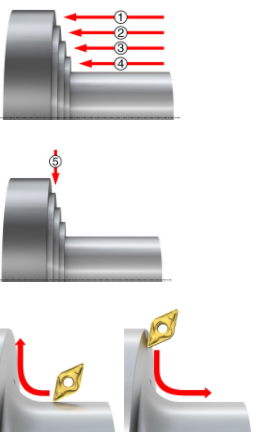
\includegraphics[width=5cm]{Figures/slanted.png}
\caption{How to create edge blends}
\label{edgeblend}
\end{figure}
\newpage